
    \begin{picture} (300.000000,185.384615)(0,0)
    \put(0.0, 0.0){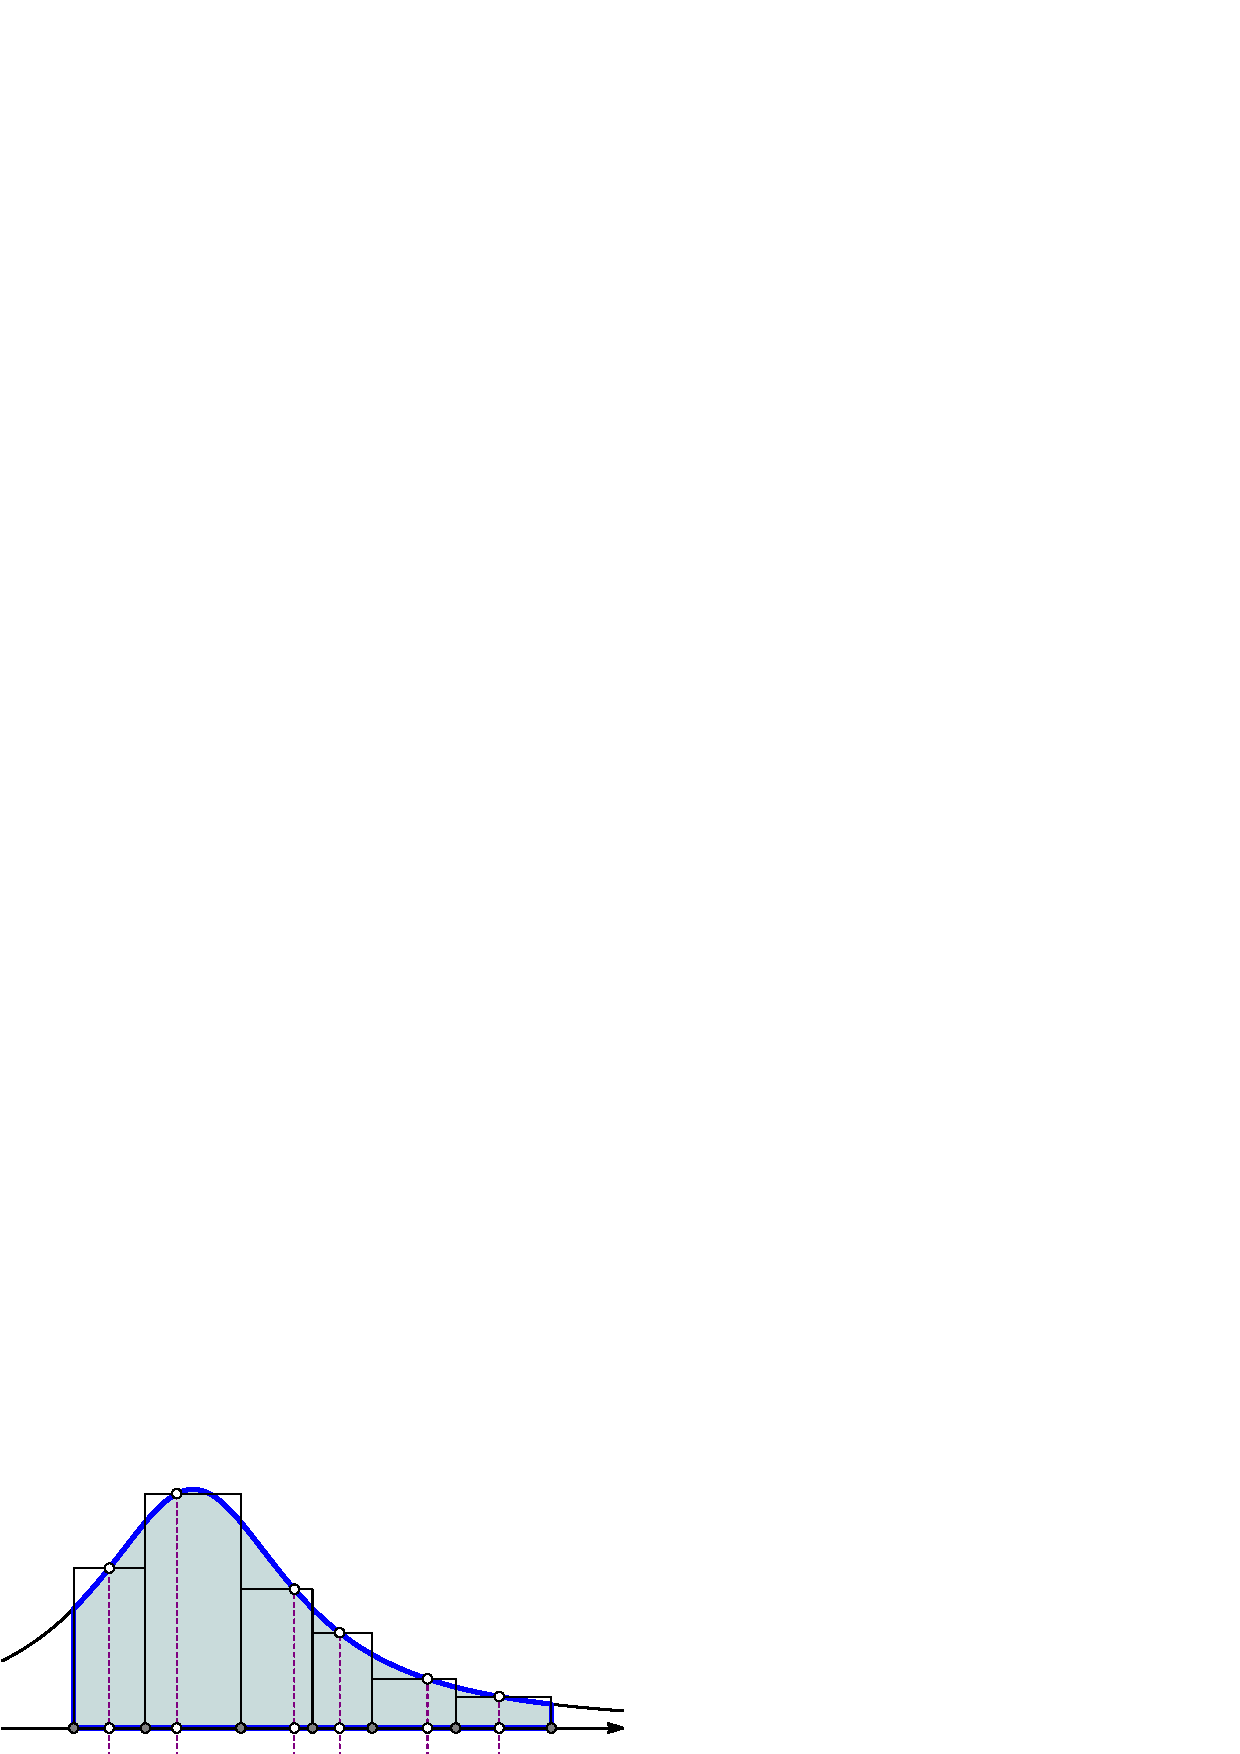
\includegraphics{08Riemann.pdf}}
        \put( 35.38,   0.46){\sffamily\itshape \makebox[0pt][r]{$a=x_0$}}
    \put( 52.45, -11.54){\sffamily\itshape \makebox[0pt][c]{$c_1$}}
    \put( 69.77,   0.46){\sffamily\itshape \makebox[0pt][c]{$x_1$}}
    \put( 84.82, -11.54){\sffamily\itshape \makebox[0pt][c]{$c_2$}}
    \put(115.62,   0.46){\sffamily\itshape \makebox[0pt][c]{$x_2$}}
    \put(141.32, -11.54){\sffamily\itshape \makebox[0pt][c]{$c_3$}}
    \put(150.00,   0.46){\sffamily\itshape \makebox[0pt][c]{$x_3$}}
    \put(162.98, -11.54){\sffamily\itshape \makebox[0pt][c]{$c_4$}}
    \put(178.65,   0.46){\sffamily\itshape \makebox[0pt][c]{$x_4$}}
    \put(205.20, -11.54){\sffamily\itshape \makebox[0pt][c]{$c_5$}}
    \put(218.77,   0.46){\sffamily\itshape \makebox[0pt][c]{$x_5$}}
    \put(239.65, -11.54){\sffamily\itshape \makebox[0pt][c]{$c_6$}}
    \put(264.62,   0.46){\sffamily\itshape \makebox[0pt][l]{$b=x_6$}}
\end{picture}
